\section{Compressed Sensing Image Reconstruction for MeerKAT} \label{intro}
An instrument in the real world measures noisy data. Measurements are corrupted by noise, interference sources or the measurement instrument itself. Image reconstruction problems appear when one tries to remove the corruption from the measurements and tries to find the observed image of the instrument. This leads to an ill-posed inverse problem: A small change in the measurements may create very different image reconstructions, and many possible images match the measurements. An image reconstruction algorithm therefore has to find the observed image from a potentially large set of possible images.

In the past, image reconstructions applied simple heuristics and approximated a likely image. How close the approximation was to the observed image was in general not known. The theory of compressed sensing\cite{candes2006robust}\cite{donoho2006compressed} introduced a new theoretical framework under which image reconstructions can be analysed. This has lead rise to new compressed sensing reconstruction algorithms, which under the right conditions are guaranteed to reconstruct the observed image. Furthermore they have shown super-resolution performance in real-world environments, creating reconstructions above the accuracy limit of the instrument.

This work applies compressed sensing image reconstruction to the field of radio astronomy. The new MeerKAT radio interferometer poses a reconstruction problem on a new scale of data volume. The raw measurements easily take up several terabytes of disk space. The focus of this work is creating a scalable compressed sensing image reconstruction algorithm.

The current state of the art reconstruction algorithm for MeerKAT is based on CLEAN\cite{rich2008multi}\cite{rau2011multi}. It is a reconstruction using a simple heuristic and was developed before the theory of compressed sensing was known. In recent years, compressed sensing reconstruction algorithms were developed for radio interferometers\cite{girard2015sparse}\cite{dabbech2018cygnus}\cite{birdi2018sparse}. They beat CLEAN in terms of reconstruction quality, producing super-resolved reconstructions. However, CLEAN has the upper hand in runtime complexity. Therefore, an efficient implementation of CLEAN is still the go to reconstruction algorithm for MeerKAT data.

The efficient implementation use CLEAN in the Major Cycle Architecture, which was developed with CLEAN in mind. Current compressed sensing algorithms use a similar architecture. So far, little research has gone into different architectures for compressed sensing reconstructions in radio astronomy. This work explores different architectures for compressed sensing reconstructions with the hope of reducing the computational complexity. 

A new proof-of-concept reconstruction algorithm was developed with a simplified architecture. It was tested on simulated MeerKAT data and the lower-bound asymptotic complexity was evaluated. The new algorithm scales independently of the image size, but scales worse with the number of input measurements compared to CLEAN. For the MeerKAT image reconstruction, the number of input measurements tends to be the largest of all numbers in the problem. Even though the algorithm could be improved further, it is unlikely to beat CLEAN reconstructions in terms of runtime complexity on MeerKAT data.

%something something measurement equation

\subsection{The basic Measurement Equation of a radio interferometry}\label{intro:basic}
Real world radio interferometers have complicated measurement equations. They become even more complicated for large interferometers like MeerKAT. These problems get addressed in section \ref{meerkat}. This section looks at the basic measurement equation of a radio interferometer \eqref{intro:measurement} and discusses the two fundamental challenges for radio interferometry image reconstruction. 

\begin{equation}\label{intro:measurement}
V(u, v) = \int\int I(x, y) e^{2 \pi i (ux+vy)} \: dx \: dy
\end{equation}

An interferometer measures Fourier Components $V$ (called Visibilities in Radio Astronomy) from the sky image $I$ at position $x$ and $y$. The term $e^{2 \pi i (ux+vy)}$ represents the two dimensional Fourier Transform. The task is to reconstruct the observed image $I$ from the measured Visibilities $V$. In theory this task is trivial: Since the inverse Fourier Transform exists, we can reconstruct the image $I$ by calculating the inverse Fourier Transform of $V$. However, two properties of the Visibilities make this task challenging in practice:

\begin{enumerate}
	\item Non-uniform sampling pattern in Visibility space
	\item Incomplete Visibility coverage. 
\end{enumerate} 

\textit{Property 1:} We want to reconstruct an image with uniformly spaced pixels. The instrument defines the sampling pattern in Visibility space and does not correspond to the exact pixels of the reconstructed image. This property keeps us from using the Fast Fourier Transform. The naive inverse Fourier Transform can still be calculated, but it has a quadratic runtime and does not scale to the data volume of interferometers. Current reconstruction algorithms use the non-uniform Fast Fourier Transform. The non-uniform FFT approximates the non-uniform Fourier Transform. 

\textit{Property 2:} Interferometers sample only a limited set of Visibilities. It does not have all information for reconstruction. When the inverse Fourier Transform is applied on the Visibilities, the resulting image is corrupted by the incomplete Visibilities. It contains structures which where introduced by the interferometer and were not observed. With only knowing the incomplete set of Visibilities a reconstruction algorithm has to decide which image structures were truly measured, and which are due to the instrument. This forms an ill-posed inverse problem. There are many images that fit the measurements, and a small change in the Visibilities can lead to a very different reconstruction. 

CLEAN represents the instrumental effect with a Point Spread Function (PSF). After the non-uniform FFT produced the 'dirty' image, CLEAN tries to reconstruct observed image with a deconvolving the 'dirty' image with the PSF. Note however that both CLEAN nor the non-uniform FFT are approximations. In real world reconstructions, these two approximations are used in the major cycle architecture to increase the reconstruction accuracy. 

%The CLEAN algorithms approximate the observed image with a deconvolution: The inverse Fourier Transform produces a corrupted image. The observed image was convolved with a known Point Spread Function (PSF), which represents the instrument corruption. Finding a deconvolution reconstructs the observed image. The deconvolution is still an ill-posed problem, there are potentially many possible deconvolutions, and a small change in the input can lead to a very different output. Furthermore the CLEAN algorithms produce a greedy approximation of the deconvolution. 


\subsection{The Major Cycle Architecture}
Major cycle was created with CLEAN in mind. Compressed sensing reconstructions use essentially the same architecture with minor modifications. 

A CLEAN image reconstruction for radio interferometers consists of two different steps: A non-uniform FFT, which approximates the inverse Fourier Transform efficiently and an deconvolution algorithm, which approximates the instrumental effects on the image (typically based on CLEAN). These two approximations are an error source of the reconstruction. The major cycle architecture \ref{intro:major} therefore tries to iteratively minimize the errors of the non-uniform FFT and the deconvolution over several iterations.

\begin{wrapfigure}{r}{0.6\textwidth}
	\centering
	\vspace{-10pt}
	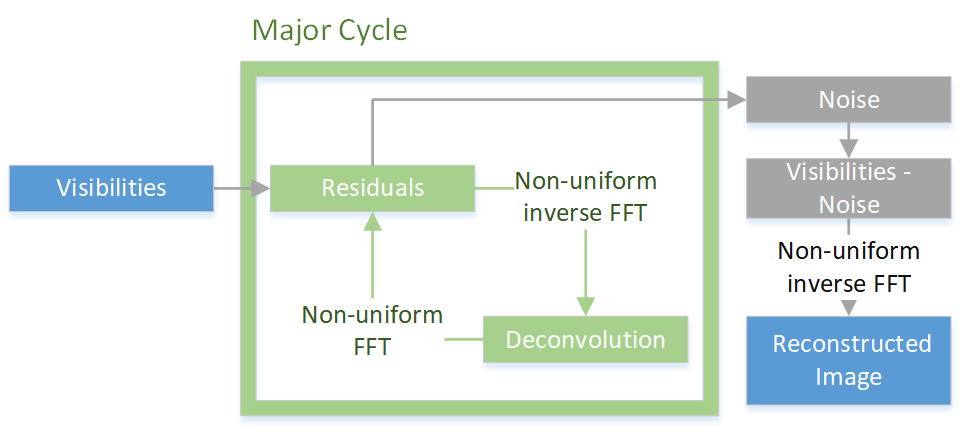
\includegraphics[width=1.0\linewidth]{./chapters/01.intro/Major-Minor.png}
	\caption{The Major Cycle Framework}
	\label{intro:major}
	\vspace{-10pt}
\end{wrapfigure}

The first major cycle uses the non-uniform inverse FFT to approximate the 'dirty' image from the Visibilities. The deconvolution algorithm decides parts which parts belong to the observed image and which are due to instrumental and other noise effects. It returns the noise part of the image, which gets transformed back into residual Visibilities. The next major cycle iteration continues with the residual Visibilities. The residual Visibilities get minimized until they contain only the instrumental effects and noise.

After several major cycles the residual  on a regularly spaced image which has a small error from non-uniform samples, and a small error from incomplete measurements.

Compressed sensing reconstructions essentially use the same architecture, although with minor alterations. In general, they keep a similar scheme of forward/backward non-uniform FFT, but do not use a deconvolution in image pace. Instead, they analyse constraints defined on the image (For example all pixels should be non-negative), and try to find the Visibilities that minimize the constraint violations.

For CLEAN reconstructions, the forward/backward non-uniform FFT are the most expensive operations, while the deconvolution is negligible. The compressed sensing algorithms tend to require more major cycle iterations to converge and the image constraint analysis tends to be more expensive than CLEAN deconvolutions. Current research into compressed sensing reconstructions is focussed on reducing the number of major cycles\cite{dabbech2018cygnus}. 

%Different architecture, but has to somehow handle all the difficulties that arise from imaging meerkat data.


%compressed sensing got rid of the miinor cycle, but essentially kept the major cycle framework
%have to handle own problems in a new architecture






